\documentclass{article}

\usepackage{times}
\usepackage{geometry}
\geometry{a4paper,left=0.6cm,right=0.7cm,top=1.5cm,bottom=1cm,columnsep=0.8cm}

\usepackage{fontawesome}          % icônes de base seulement
\usepackage[hidelinks]{hyperref}
\usepackage{multicol}
\usepackage{tikz}
\usepackage{hyphsubst}
\usepackage{moresize}
\usepackage{hyphenat}
\usepackage{tabularx}
\usepackage{ragged2e}
\usepackage{xcolor}
\usepackage{enumitem}
\usetikzlibrary{calc, positioning}
\newcolumntype{Y}{>{\RaggedRight\arraybackslash}X}

% icônes manquantes -> puce
\makeatletter
\@for\sym:=faBrain,faMicrochip,faHandshakeO,faTools,faNetworkWired,%
             faDatabase,faServer,faGit,faUsers,faComments,faCalendar,faGroup\do{%
  \@ifundefined{\sym}{\expandafter\newcommand\csname\sym\endcsname{\textbullet}}{}}
\makeatother

% couleurs
\definecolor{maincolor}{HTML}{f0fafc}
\definecolor{seccolor}{HTML}{ffffff}
\definecolor{gray}{HTML}{8c94a9}
\definecolor{sidetext}{HTML}{59cee5}

% bande latérale bleue
\usepackage{eso-pic}
\AddToShipoutPictureBG{%
  \begin{tikzpicture}[remember picture,overlay]
    \fill[maincolor] (current page.north west) rectangle
                     ([xshift=0.3\paperwidth] current page.south west);
  \end{tikzpicture}%
}

% listes
\setlist[itemize]{itemsep=-2pt,topsep=0pt,leftmargin=1.08cm}
\renewcommand{\labelitemi}{\textcolor{sidetext}{\footnotesize$\bullet$}}

\setlength{\parindent}{0pt}
\usepackage{paracol}
\columnratio{0.3}

\begin{document}
\pagestyle{empty}

\begin{paracol}{2}
% ────────────────────────────────────────
% Colonne gauche
% ────────────────────────────────────────
\color{sidetext}
\vspace*{-0.5cm}

\noindent
\begin{minipage}{\linewidth}
  \centering
  \begin{tikzpicture}
    \clip (0,0) circle (1.5cm) node[anchor=center]
      {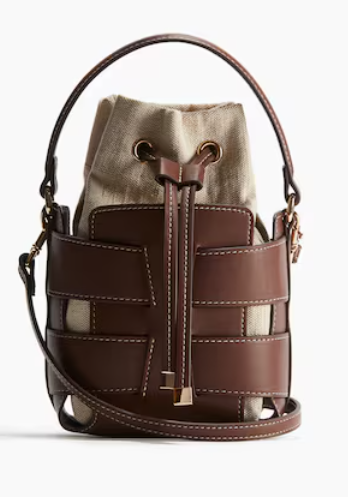
\includegraphics[width=3cm]{dc7e06b574f04f0c978a4c609bbf9e99.png}};
  \end{tikzpicture}

  \vspace{3mm}
  {\color{black}\LARGE \textbf{Mourouvin Judikael}}

  \vspace{1mm}
  {\large Technicien informatique \& marketing digital}

  \vspace{3mm}
  {\color{gray}\rule{\linewidth}{0.4pt}} \\
\end{minipage}

% ── Coordonnées
\begin{tabular}{@{}c l}
  \faPhone &
  \begin{tabular}[t]{@{}l@{}}
    {\color{gray}Téléphone} \\ +590690911448
  \end{tabular} \\
  \\
  \faLinkedin &
  \begin{tabular}[t]{@{}l@{}}
    {\color{gray}LinkedIn} \\
    \href{}{Mon LinkedIn}
  \end{tabular} \\
  \\
  \faMapMarker &
  \begin{tabular}[t]{@{}l@{}}
    {\color{gray}Adresse} \\ Route de Cocoyer \\ 97190 Le Gosier
  \end{tabular} \\
  \\
  \faEnvelope &
  \begin{tabular}[t]{@{}l@{}}
    {\color{gray}Email} \\
    \href{mailto:jkmou971@gmail.com}{jkmou971@gmail.com}
  \end{tabular} \\
\end{tabular}

\vspace{2mm}
{\color{gray}\rule{\linewidth}{0.4pt}} \\

% ── Langues --------------------------------------------------------
{\color{black}{Langues}}

\vspace{2mm}
\begin{itemize}[leftmargin=*]
\item English - \textcolor{gray}{}
\item Espagnol - \textcolor{gray}{}\end{itemize}          % ← le placeholder va contenir \begin{itemize}…\end{itemize}

{\color{gray}\rule{\linewidth}{0.4pt}} \\

% ── Compétences ----------------------------------------------------
\vspace{2mm}
{\color{black}{Compétences Clés}}

\vspace{2mm}
\begin{itemize}[leftmargin=*]
\item Réseaux
\item Support
\item Maintenance
\item Marketing
\item Diagnostic
\item Configuration
\item Assistance\end{itemize}              % ← idem, une vraie liste
\vspace{2mm}
{\color{gray}\rule{\linewidth}{0.4pt}} \\

% ── Centres d'intérêt
\vspace{2mm}
{\color{black}{Centres d’intérêt}}

\vspace{2mm}
\begin{itemize}[leftmargin=*]
\item Lectur
\item Sports
\item Musique
\item Voyage
\end{itemize}     % ← simple itemize ou tabular

\vfill
~

% ────────────────────────────────────────
\switchcolumn
% Colonne droite
% ────────────────────────────────────────
\color{black}

% ── Profil
\textcolor{black}{\Large \textbf{Profil Professionnel}} \\[2pt]
Passionné par l’informatique et le marketing digital, je maîtrise la configuration de postes, la maintenance matérielle et le support aux utilisateurs. Mon année d’alternance à la DSI de la Mairie du Gosier m’a permis de contribuer à des projets numériques et de développer une approche orientée résultats. Rigoureux et méthodique, je sais analyser les besoins, déployer des solutions adaptées et accompagner les usagers dans leur adoption. Je souhaite désormais mettre ces compétences au service de votre organisation à temps plein. \\[8pt]

% ── Expérience
\textcolor{black}{\Large \textbf{Expérience Professionnelle}} \\[2pt]

\colorbox{maincolor}{%
  \begin{minipage}{\linewidth}
    \textbf{Alternant en Marketing Digital}   2023-2024  \\ Mairie du Gosier – DSI 
    \begin{itemize}
      \item Piloté des projets numériques et assuré leur déploiement conforme aux attentes \item Analysé les besoins des utilisateurs puis déployé des solutions adaptées et pérennes \item Assuré support et formations, renforçant l’adoption des outils digitaux
    \end{itemize}
  \end{minipage}}

\vspace{3mm}


\colorbox{maincolor}{%
  \begin{minipage}{\linewidth}
    \textbf{Animateur de la zone informatique}   2022-2023  \\ Pôle Emploi, Le Gosier 
    \begin{itemize}
      \item Assuré l’assistance quotidienne des utilisateurs pour résoudre leurs demandes \item Configuré et entretenu les postes de travail pour garantir leur disponibilité \item Diagnostiqué et résolu les incidents afin de limiter les interruptions de service
    \end{itemize}
  \end{minipage}}

\vspace{3mm}


\colorbox{maincolor}{%
  \begin{minipage}{\linewidth}
    \textbf{Stagiaire Informaticien}   2020-2021  \\ Numerika, Baie-Mahault 
    \begin{itemize}
      \item Configuré et maintenu les équipements informatiques pour optimiser leurs performances \item Fournit un support de proximité aux utilisateurs, améliorant leur efficacité quotidienne
    \end{itemize}
  \end{minipage}}   % ← blocs \colorbox{maincolor}{\begin{minipage}…}

\vspace{8mm}

% ── Formation
\textcolor{black}{\Large \textbf{Formation}} \\[2pt]

\begin{tabularx}{\linewidth}{@{}c  >{\RaggedRight\arraybackslash}X
                             >{\raggedleft\arraybackslash}p{0.25\linewidth}@{}}
\textcolor{sidetext}{\faGraduationCap} &
Bachelor Marketing Digital &
2023-2024 \\
& CFA IUTS & \\   % ligne de l’établissement
\end{tabularx}
\begin{itemize}[leftmargin=*]
  \item Stratégies de communication et acquisition en ligne
  \item Gestion de projets digitaux et analyse de données marketing 
  \item Création de contenus et optimisation du référencement
\end{itemize}
\vspace{3mm}

\begin{tabularx}{\linewidth}{@{}c  >{\RaggedRight\arraybackslash}X
                             >{\raggedleft\arraybackslash}p{0.25\linewidth}@{}}
\textcolor{sidetext}{\faGraduationCap} &
BTS Système Numérique – Informatique et Réseaux &
2019-2021 \\
& Lycée Chevalier Saint-Georges, Les Abymes & \\   % ligne de l’établissement
\end{tabularx}
\begin{itemize}[leftmargin=*]
  \item Architecture des réseaux et administration systèmes
  \item Maintenance matérielle et logicielle des équipements
  \item Support technique et gestion des incidents
\end{itemize}       % ← lignes tabular par diplôme

\end{paracol}
\end{document}

